
\documentclass[tikz, border=10pt]{standalone}
\usepackage{tikz}
\usetikzlibrary{positioning, chains, shapes.geometric, fit, shapes, arrows.meta, calc, backgrounds}

\begin{document}
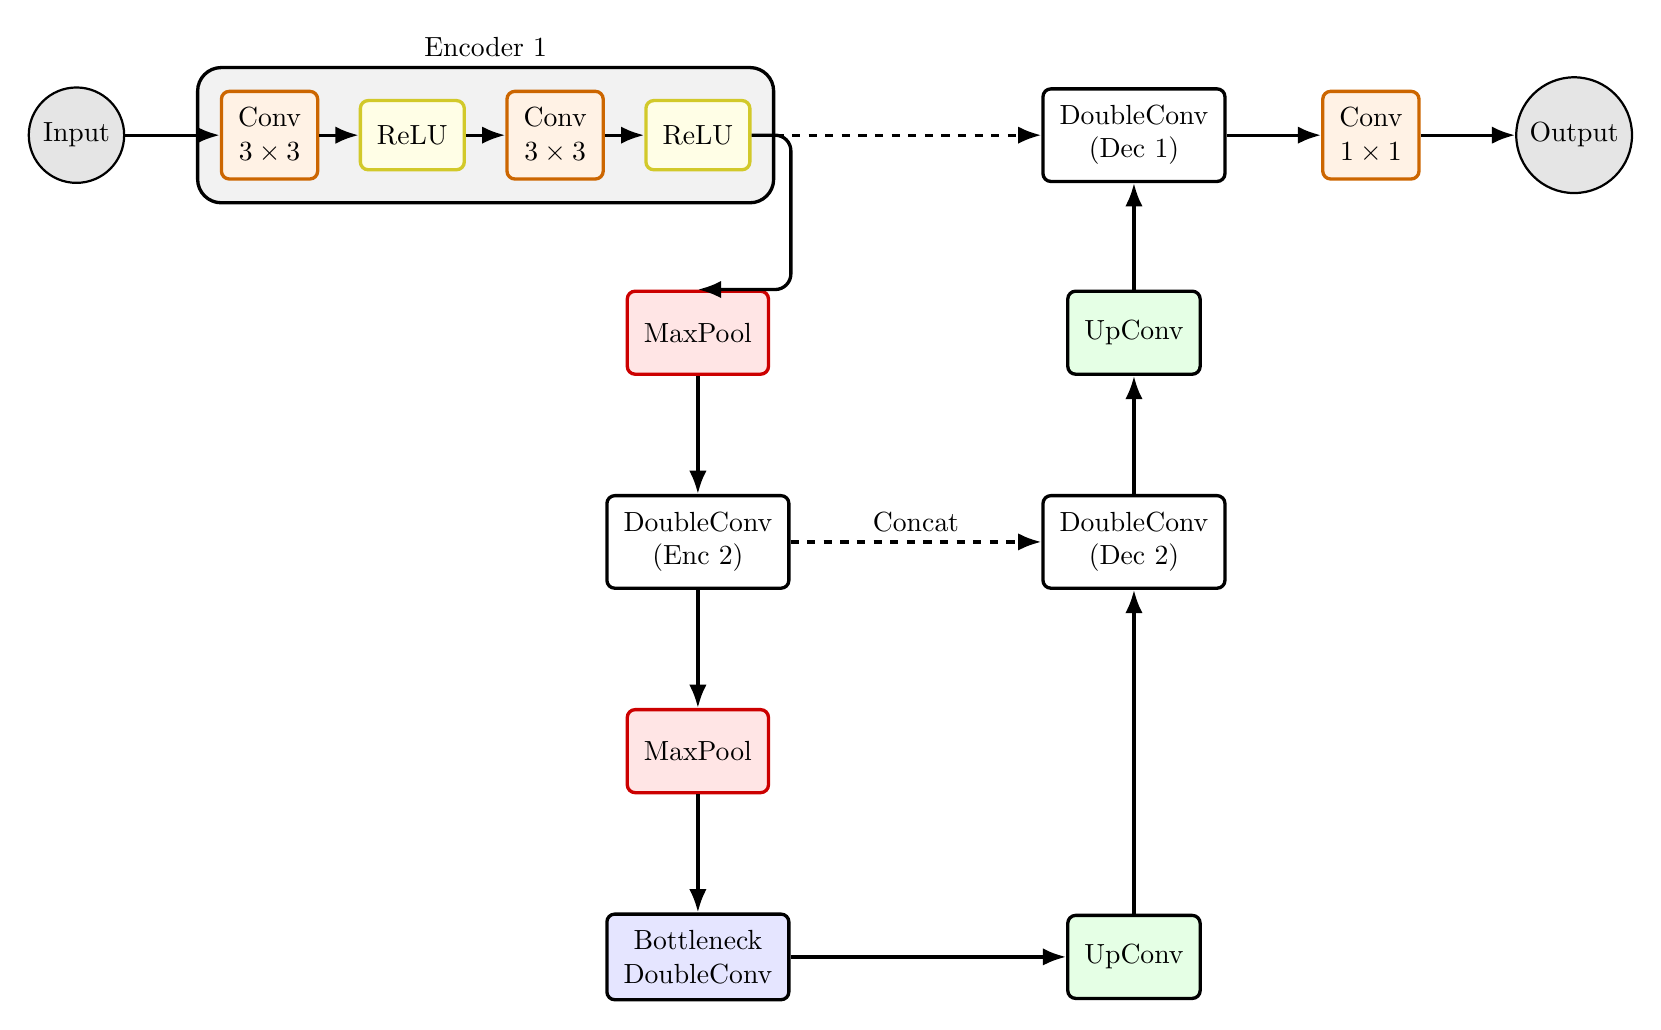
\begin{tikzpicture}[
    >=LaTeX, 
    very thick,
    node distance=1.0cm and 1.2cm,
    arrow/.style={
        ->,
        very thick,
        rounded corners=0.2cm
    },
    block/.style={
        rectangle,
        fill=gray!10,
        rounded corners=3mm,
        draw,
        very thick,
        inner sep=0.8em
    },
    layer/.style={
        rectangle,
        fill=white!10,
        rounded corners=1mm,
        inner xsep=0.6em,
        inner ysep=0.6em,
        minimum height=3.0em,
        align=center,
        draw,
        very thick
    },
    conv/.style={
        layer,
        fill=orange!10,
        draw=orange!80!black
    },
    relu/.style={
        layer,
        fill=yellow!10,
        draw=yellow!80!black,
        minimum height=2.5em
    },
    pool/.style={
        layer,
        fill=red!10,
        draw=red!80!black
    },
    input/.style={ 
        circle,
        minimum width=3.0em,
        draw,
        fill=gray!20,
        thick,
        align=center
    },
    sum/.style={
        circle,
        draw,
        fill=white,
        inner sep=0pt,
        minimum size=1.2em,
        node contents={+}
    }
]


    % Input
    \node[input] (in) {Input};

    % Encoder 1 (Detailed)
    \node[conv, right=of in] (enc1_c1) {Conv\\$3\times 3$};
    \node[relu, right=0.5cm of enc1_c1] (enc1_r1) {ReLU};
    \node[conv, right=0.5cm of enc1_r1] (enc1_c2) {Conv\\$3\times 3$};
    \node[relu, right=0.5cm of enc1_c2] (enc1_r2) {ReLU};
    
    \begin{scope}[on background layer]
        \node[block, fit=(enc1_c1) (enc1_r2), label=above:Encoder 1] (enc1) {};
    \end{scope}
    
    \draw[arrow] (in) -- (enc1_c1);
    \draw[arrow] (enc1_c1) -- (enc1_r1);
    \draw[arrow] (enc1_r1) -- (enc1_c2);
    \draw[arrow] (enc1_c2) -- (enc1_r2);

    % Pool 1 (Aligned below enc1_r2 to avoid backtracking)
    \node[pool, below=1.5cm of enc1_r2] (pool1) {MaxPool};
    % Path from rightmost encoder node to pool
    \draw[arrow] (enc1_r2.east) -- ++(0.5,0) |- (pool1.north);

    % Encoder 2 (Aligned with Encoder 1 end)
    \node[layer, below=1.5cm of pool1] (enc2) {DoubleConv\\(Enc 2)};
    \draw[arrow] (pool1) -- (enc2);

    % Bottleneck
    \node[pool, below=1.5cm of enc2] (pool2) {MaxPool};
    \draw[arrow] (enc2) -- (pool2);
    
    \node[layer, below=1.5cm of pool2, fill=blue!10] (bot) {Bottleneck\\DoubleConv};
    \draw[arrow] (pool2) -- (bot);

    % --- Decoder Side (Strict Alignment) ---

    % Up2 (Same level as Bot, shifted right)
    \node[layer, right=3.5cm of bot, fill=green!10] (up2) {UpConv};
    \draw[arrow] (bot) -- (up2);

    % Dec2 (Aligned with Enc2)
    \node[layer, at={(up2 |- enc2)}] (dec2) {DoubleConv\\(Dec 2)};
    \draw[arrow] (up2) -- (dec2);

    % Skip Connection 2 (Horizontal)
    \draw[arrow, dashed] (enc2.east) -- node[above]{Concat} (dec2.west);

    % Up1 (Aligned with Pool1 level)
    \node[layer, at={(dec2 |- pool1)}, fill=green!10] (up1) {UpConv};
    \draw[arrow] (dec2) -- (up1);

    % Dec1 (Aligned with Enc1 output / Enc1 level)
    \node[layer, at={(up1 |- enc1)}] (dec1) {DoubleConv\\(Dec 1)};
    \draw[arrow] (up1) -- (dec1);

    % Skip Connection 1 (Horizontal-ish)
    \draw[arrow, dashed] (enc1.east) -- (dec1.west);

    % Output
    \node[conv, right=1.2cm of dec1] (out_conv) {Conv\\$1\times 1$};
    \node[input, right=of out_conv] (out) {Output};
    
    \draw[arrow] (dec1) -- (out_conv);
    \draw[arrow] (out_conv) -- (out);

\end{tikzpicture}
\end{document}
